\documentclass[10pt,a4paper]{article}
\usepackage[utf8]{inputenc}
\usepackage{amsmath}
\usepackage{amsfonts}
\usepackage{amssymb}
\usepackage{verbatim}
\usepackage{graphicx}
\usepackage{listings}
\usepackage{xcolor}

\lstdefinestyle{matlabcode}{
  language=Matlab,
  basicstyle=\ttfamily\small,
  keywordstyle=\color{blue},
  commentstyle=\color{green!50!black},
  stringstyle=\color{red},
  frame=single,
  breaklines=true,
  breakatwhitespace=false,
  tabsize=2,
  showstringspaces=false
  inputencoding = utf8,  % Input encoding
  extendedchars = true,  % Extended ASCII
  literate={é}{{\'e}}1 {è}{{\`e}}1 {à}{{\`a}}1 {ù}{{\`u}}1 {ò}{{\`o}}1
}
\lstset{basicstyle=\tiny, style=matlabcode}

\author{Alessio Santoro (7029440) - Lorenzo Campinoti (7030227)}
\title{Elaborato Calcolo Numerico}
\date{A.A. 2022/2023}
\begin{document}
\maketitle 	
\textbf{Nota}: Per gli esercizi che prevedono delle \textit{funcion} Matlab, si specifica nella relativa risposta al quesito i file tra gli alleagti a cui essa si riferisce.
\section{}
Si considera lo sviluppo delle funzioni $f(x-h), f(x+h), f(x+2h), f(x+3h)$:
\begin{align*}
&f(x-h)=f(x)-hf'(x)+\frac{h^2}{2}f''(x)-\frac{h^3}{6}f^{(3)}(x)+\frac{h^4}{24}f^{(4)}(x)+O(h^5)\\&f(x+h)=f(x)+hf'(x)+\frac{h^2}{2}f''(x)+\frac{h^3}{6}f^{(3)}(x)+\frac{h^4}{24}f^{(4)}(x)+O(h^5)\\&f(x+2h)=f(x)+2hf'(x)+\frac{4h^2}{2}f''(x)+\frac{8h^3}{6}f^{(3)}(x)+\frac{16h^4}{24}f^{(4)}(x)+O(h^5)\\&f(x+3h)=f(x)+3hf'(x)+\frac{9h^2}{2}f''(x)+\frac{27h^3}{6}f^{(3)}(x)+\frac{81h^4}{24}f^{(4)}(x)+O(h^5)
\end{align*}
Si sostiuiscono le espressioni così trovate nella parte sinistra dell'equaziome iniziale e si ottiene la seguente espressione:
\begin{align*}
&-\frac{1}{4}\left[f(x)-hf'(x)+\frac{h^2}{2}f''(x)-\frac{h^3}{6}f^{(3)}(x)+\frac{h^4}{24}f^{(4)}(x)+O(h^5)\right]+\\&-\frac{5}{6}\left[f(x)\right]+\\&+\frac{3}{2}\left[f(x)+hf'(x)+\frac{h^2}{2}f''(x)+\frac{h^3}{6}f^{(3)}(x)+\frac{h^4}{24}f^{(4)}(x)+O(h^5)\right]+\\&-\frac{1}{2}\left[f(x)+2hf'(x)+\frac{4h^2}{2}f''(x)+\frac{8h^3}{6}f^{(3)}(x)+\frac{16h^4}{24}f^{(4)}(x)+O(h^5)\right]+\\&+\frac{1}{12}\left[f(x)+3hf'(x)+\frac{9h^2}{2}f''(x)+\frac{27h^3}{6}f^{(3)}(x)+\frac{81h^4}{24}f^{(4)}(x)+O(h^5)\right]
\end{align*}
Si procede a moltiplicare i coefficienti di ogni espressione e poi raccogliere i termini che contengono le derivate dello stesso ordine, una volta raccolti i temrini assumono i seguenti valori che, stando all'equazione iniziale dovranno poi essere sommati:
\begin{align}
f(x)\left[-\frac{1}{4}-\frac{5}{6}+\frac{3}{2}-\frac{1}{2}+\frac{1}{12}\right]=0\\	f'(x)\cdot h\left[\frac{1}{4}+\frac{3}{2}-\frac{1}{2}2+\frac{1}{12}3\right]=hf'(x)\\f''(x)\cdot\frac{h^2}{2}\left[-\frac{1}{4}+\frac{3}{2}-\frac{1}{2}4+\frac{1}{12}9\right]=0\\f^{(3)}(x)\cdot\frac{h^3}{6}\left[-\frac{1}{4}+\frac{3}{2}-\frac{1}{2}8+\frac{1}{12}27\right]=0\\f^{(4)}(x)\cdot\frac{h^4}{24}\left[-\frac{1}{4}+\frac{3}{2}-\frac{1}{2}16+\frac{1}{12}81\right]=0
\end{align}
Dalle espressioni (1)...(5) e dalle proprietà degli "O-grande" di moltiplicazione per una costante segue l'asserto.
\section{}
La doppia precisione dello standard IEEE 754 è una rappresentazione in base binaria, in forma normalizzata ($1.f$) che approssima per arrotondamento e occupa 64 bit, di cui 52 dedicati alla frazione (53 alla mantissa).\\Si può dunque ottenere il valore della precisione di macchina ($u$) dalla seguente espressione, dove: $b=2$ rappresenta la base, e $m=53$ la mantissa:$$u = \frac{1}{2}b^{1-m} = 2^{-53}$$
Invece \texttt{eps} è definito dalla stessa funzione \texttt{help} di Matlab come 	la distanza tra \texttt{1.0} e il maggior valore a doppia precisione successivo disponibile, ovvero $ 2^{-52} $.
Si osserva infatti che, considerato il valore $x = 1+u = 1+2^{-53}\neq 1 $ e sia \textit{fl} la funzione di floating, allora vale che $fl(x)=1 $, poichè $u=2^{-53}<2^{-52}=$\texttt{eps}.\\Vi è dunque un errore di rappresentazione del valore \textit{x} ($\varepsilon_x$), determinato dalla seguente espressione:$$\varepsilon_x=\frac{|x-fl(x)|}{|x|}=\frac{|1+2^{-53}-1|}{|1+2^{-53}|}=\frac{|2^{-53}|}{|1+2^{-53}|}<|2^{-53}|=u$$
\section{}La cancellazione numerica è quel fenomeno in cui, sommando in aritmetica finita due numeri quasi opposti si verifica la perdita di cifre signficative. Questo è dovuto all'espressione del numero di condizionamento della somma in aritmetica finita ($k$) che per due valori $x$ e $y$ è dato da:$$k = \frac{|x|+|y|}{|x+y|}$$Infatti, se $x\rightarrow-y$ allora $k\rightarrow\infty$ e la somma tra $x$ e $y$ risulta mal condizionata.
\section{}
Sia $x^*\in\mathbb{R}$ il valore di cui si ricerca la radice sesta.\\
Per calcolarlo si definisce una funzione $f(x)$ come segue:
$$f(x) = x^6-x^*$$La cui derivata è:$$f'(x)=6x^5$$La funzione $f(x)$ si annulla solo nella radice sesta di $x^*$, quindi avendo un'approsimazione iniziale $x_0$ si può applicare il metodo di Newton alla funzione $f(x)$ per ricercarne una radice che coinciderà con il valore cercato:
$$x_{i+1}=x_i+\frac{f(x_i)}{f'(x_i)}=x_i-\frac{x_i^6-x^*}{6x_i^5}=\frac{1}{6}\left[5x_i+\frac{x^*}{x_i}\right]$$
La \texttt{function} che implementa il metodo presentato è contenuta nel file \texttt{radice.m}:

\lstinputlisting{../functions/4/radice.m}


\pagebreak
I dati sul confronto tra il  risultato offerto dalla funzione e il valore \texttt{x\^ (1/6)} sono contentuti nel file \texttt{4\_table.txt}:
\verbatiminput{../tables/4_table.txt}
\section{}
Il seguente testo è cotnenuto nel file \texttt{newtonMethod.m} e rappresenta il metodo di Newton:
\lstinputlisting{../functions/5/newtonMethod.m} %a
Da qui in poi viene presentato il contenuto del file \texttt{secantsMethod.m} che rappresenta il metodo delle secanti:\\
\lstinputlisting{../functions/5/secantsMethod.m}

\section{}
Nel file \texttt{6\_result.txt} è contenuta la tabella dei risultati delle funzioni precedentemente mostrate:
\verbatiminput{../tables/6\_result.txt}
Per entrambi i metodi, la parte più costosa computazionalmente è la valutazione funzionale, dato che tutte le altre operazioni che vengono svolte sono operazioni elementari.\\
Il metodo di Newton esegue due valutazioni in ogni iterazione.\\
Sia $n$ il numero di iterazioni, il costo computazionale del metodo di Newton è dato da $2(n+1)$.\\
Il metodo delle secanti esegue due valutazioni iniziali e poi una per ogni iterazione, quindi il suo costo computazionale per $n$ iterazioni è dato da $n+2$.
\begin{center}
\begin{tabular}{|c c c c c|} 
 \hline
 Tolleranza & Iterazioni Newton & Costo Newton & Iterazioni secanti & Costo secanti\\ [0.5ex] 
 \hline
 $10^{-3}$ & 8 & 16 & 4 & 6 \\ 
 \hline
 $10^{-6}$ & 9 & 18 & 6 & 8 \\
 \hline
 $10^{-9}$ & 10 & 20 & 6 & 8 \\
 \hline
 $10^{-12}$ & 10 & 20 & 7 & 9 \\
 \hline
\end{tabular}
\end{center}
\pagebreak
\section{}
La seguente tabella fornisce i risultati dell'utilizzo delle funzioni precedenti per calcolare la radice della funzione $f(x)=[x-cos(x)]^5$:\\\\
\texttt{
\begin{tabular}{|*{5}{c|}}
	\hline
	{tolleranza} &	{Newton ris.} &	{Newton iter.} &	{Secant ris.} &	{Secant iter.}\\\hline
	10e-3 & 0.74512 & 18 & 0.73015 & 26 \\ \hline
	10e-6 & 0.73909 & 49 & 0.73908 & 70 \\ \hline
	10e-9 & 0.73909 & 80 & 0.73909 & 115\\ \hline
	10e-12 & 0.73909 & 111 & 0.73909 & 159\\ \hline
\end{tabular}}
\\\\Dopo aver sviluppato la \textit{function} \texttt{modifiedNewtonMethod.m} si sono riscontrati i seguenti risultati:\\\\
\texttt{
\begin{tabular}{|*{3}{c|}} \hline
	tolleranza & risultato Newton modificato & numero di iterazioni \\\hline
	1e-3 & 0.73909 & 22 \\\hline
	1e-6 & 0.73909 & 23 \\\hline
	1e-9 & 	0.73909 & 24 \\\hline
	1e-12 & 	0.73909 & 24 \\\hline
\end{tabular}}
\\\\Come atteso, i metodi di Newton e delle secanti sono più lenti a causa del metodo di Newton modificato, a causa della natura multipla della radice.\\Infatti il metodo di Newton e quello delle secanti hanno convergenza quadratica nel caso di radici a molteplicità 1, ma solo lineare nel caso di radici multiple.\\La modifica che abbiamo fatto, ovvero $x_{i+1} = x_i-m\cdot\frac{f(x_i)}{f'(x_i)}$, nonostante richieda che la molteplcità $m$ della radice sia nota, ripristina la convergenza quadratica del metodo di Newton.\\
I rislutati sono contentuti nel file \texttt{table\_7.txt} e si mostra di seguito il codice della funztion del metodo di Newton modificato:\\
\lstinputlisting{../functions/7/modifiedNewtonMethod.m}%a
\section{}
Il codice della \textit{function} è contenuto nel file \texttt{mialu.m}:\\
\lstinputlisting{../functions/8/mialu.m}%a
Un esempio di utilizzo è contenuto nel file di testo \texttt{ex\_8\_mialu.txt}:
%Se pensi che i range per i numeri random non vadano bene sentiti libero di cambiare tutto, tanto ho solo fatto copia/incolla dalla console di matlab
\verbatiminput{../tables/ex_8_mialu.txt}%a

\section{}
Il codice della \textit{function} è contenuto nel file \texttt{mialdl.m}:\\
\lstinputlisting{../functions/9/mialdl.m}%a
Un esempio di utilizzo è contenuto nel file di testo \texttt{9\_mialdl.txt}:
%Se pensi che i range per i numeri random non vadano bene sentiti libero di cambiare tutto, tanto ho solo fatto copia/incolla dalla console di matlab
\verbatiminput{../tables/9_mialdl.txt}%a
\section{}
La funzione è nel file \texttt{functions/miaqr.m}, mostrato di seguito insieme ad un esempio in cui viene applicato:
\\
\lstinputlisting{../functions/10/miaqr.m}
\verbatiminput{../tables/10_miaqr.txt}
\pagebreak
\section{}
Di seguito un esempio di applicazione di \texttt{mialu} per risolvere i sistemi generati da \texttt{linsis}:
\verbatiminput{../tables/11_linsis_mialu_1.txt}
Il risltato sembra essere corretto, ma se si sottrae le soluzioni ad un vettore composto di soli 1, si può osservare l'errore nella risoluzione.\\
Nel sistema $A_1x=b_1$ l'errore è nell'ordine di $10^{-15}$ mentre nel secondo sistema $A_2x=b_2$ l'ordine di errore è di $10^{-6}$.\\
L'errore molto maggiore nel secondo sistema è dovuto al mal condizionamento della matrice dei coefficienti.
\verbatiminput{../tables/11_linsis_mialu_2.txt}
\section{}
Similemente a quanto si è ottenuto per l'esercizio precedente, si può osservare come i risultati ottenuti dalla funzione \texttt{mialdl} siano accurati con un oridne di grandezza dell'errore di $10^{-15}$ per il primo sistema e $10^{-6}$ per il secondo. Anche in questo caso la differenza è dovuta alla differenza del condizionamento delle due matrici $A_1$ e $A_2$.
\verbatiminput{../tables/12_linsis_mialdl.txt}
\section{}
Di seguito si mostra come sono stati assegnati i valori richiesti, le soluzioni trovate con la funzione \texttt{miaqr} sono confrontate con il risultato dell'operatore \texttt{$\backslash$}.
\verbatiminput{../tables/13\_miaqr.txt}
Si osserva come le soluzioni siano coerenti, ma la norma del vettore residuo aumenta, negli ultimi due sistemi è quasi il triplo che nel primo.\\
\section{}
La funzione è contenuta nel file \texttt{newton.m} nella cartella \texttt{14}.
\lstinputlisting{../functions/14/newton.m}%a
\section{•}
\section{}
\lstinputlisting{../functions/16/lagrange.m}
\section{}\lstinputlisting{../functions/17/newton.m}
\section{}\lstinputlisting{../functions/18/hermite.m}
\section{}\lstinputlisting{../functions/19/chebyshev.m}
\section{}
Il codice della \textit{function} è contenuto nel file \texttt{lebesgue.m}:\\
\lstinputlisting{../functions/20/lebesgue.m}

\begin{figure}[h]
  \centering
  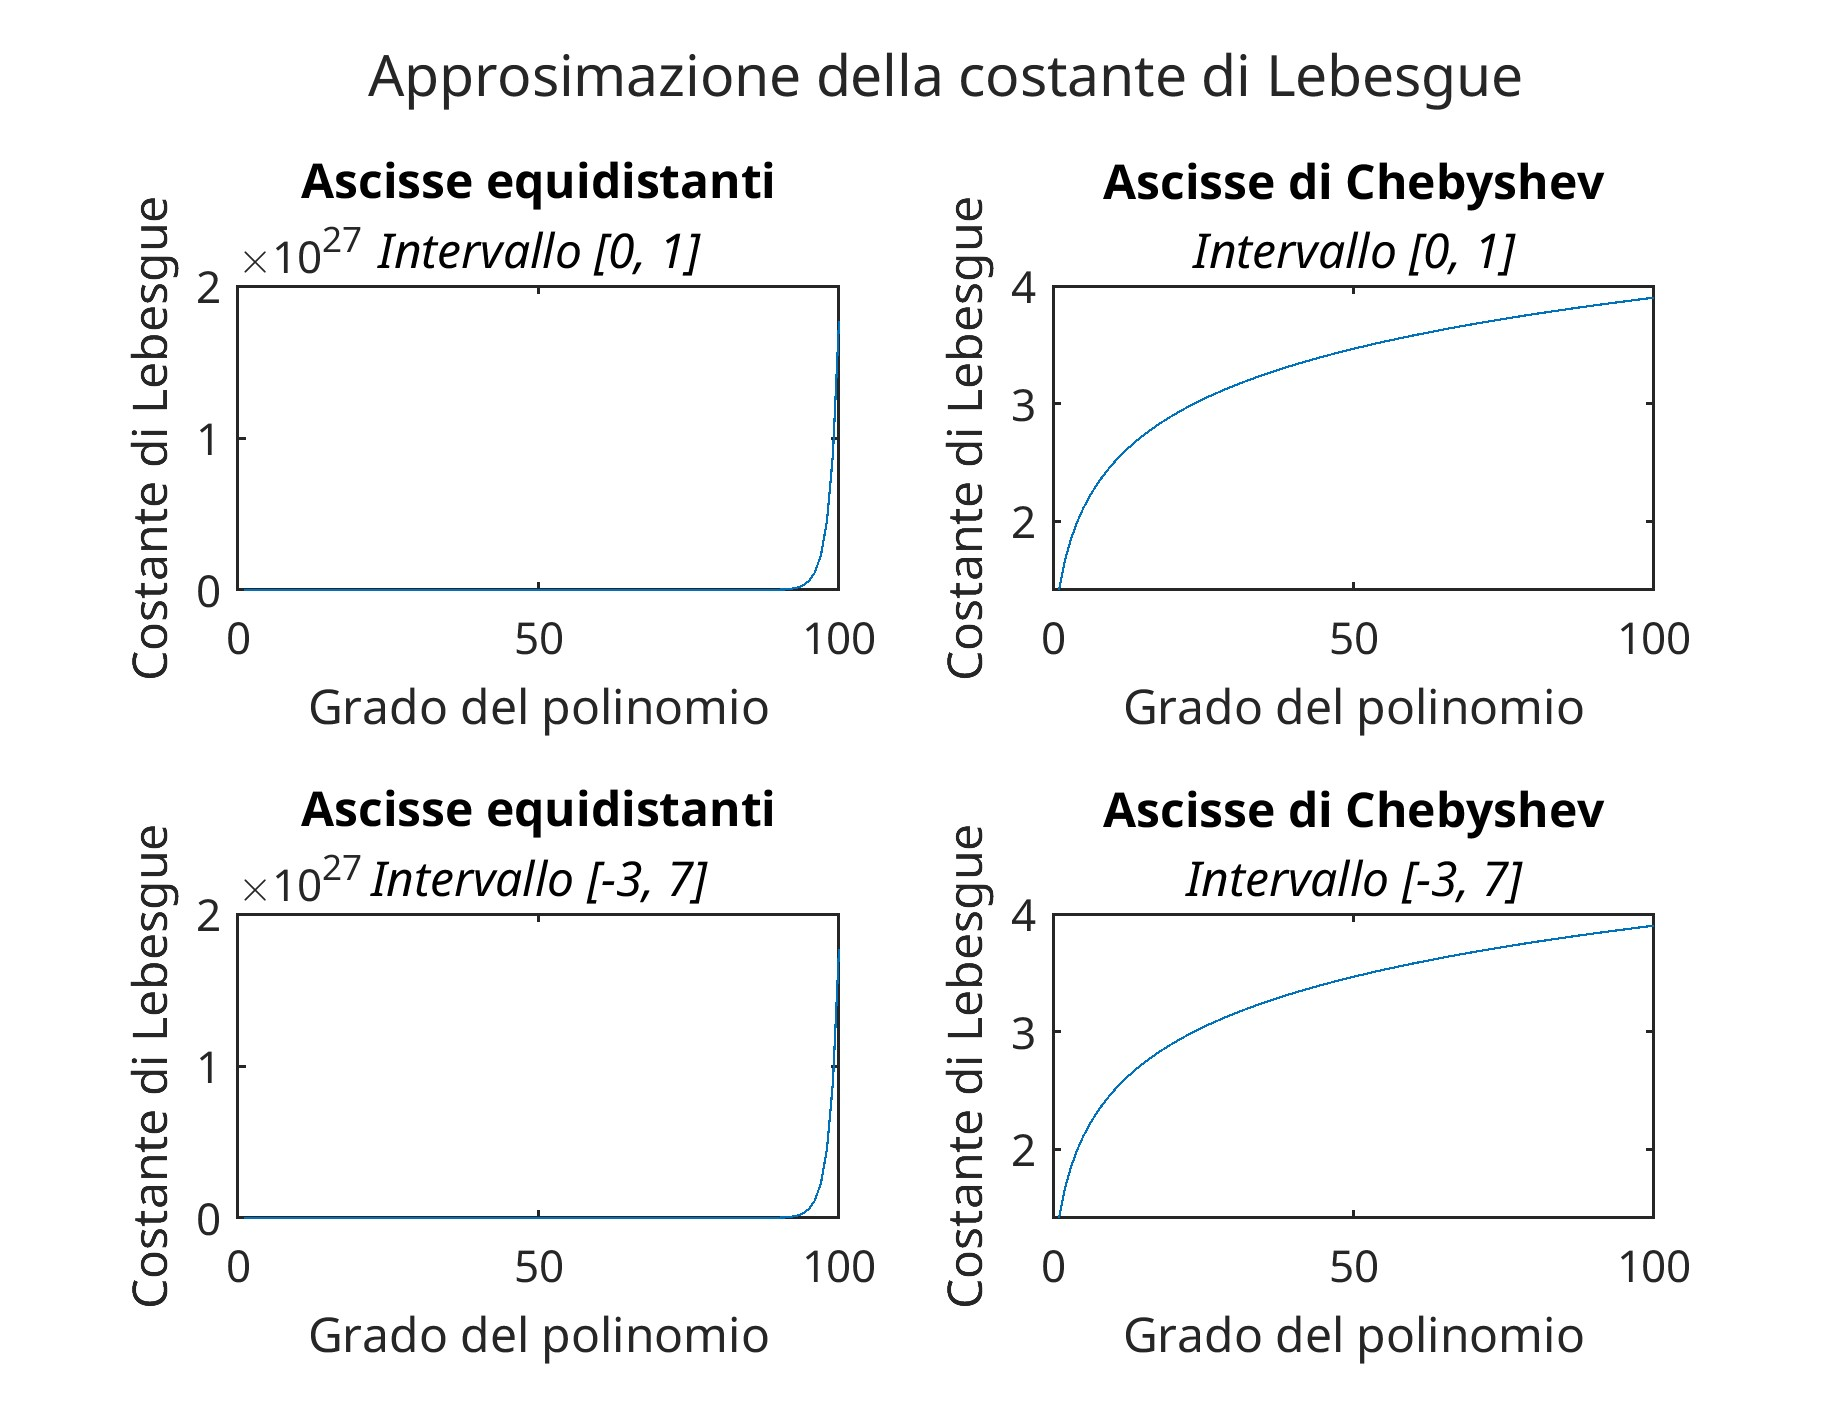
\includegraphics[width=1.1\textwidth]{../figure/plot20}  
\end{figure}


Si riportano inoltre i grafici dei risultati ottenuti per l'approssimazione della costante di Lebesgue su due intervalli distinti, si nota che il risultato è unicamente dipendente dalla scelta delle ascisse che operiamo e non dagli intervalli considerati.
\clearpage

\section{}

Grafici in scala semilogaritmica degli errori di interpolazione commessi dai vari algoritmi di interpolazione.
\begin{figure}[h!]
  \centering
  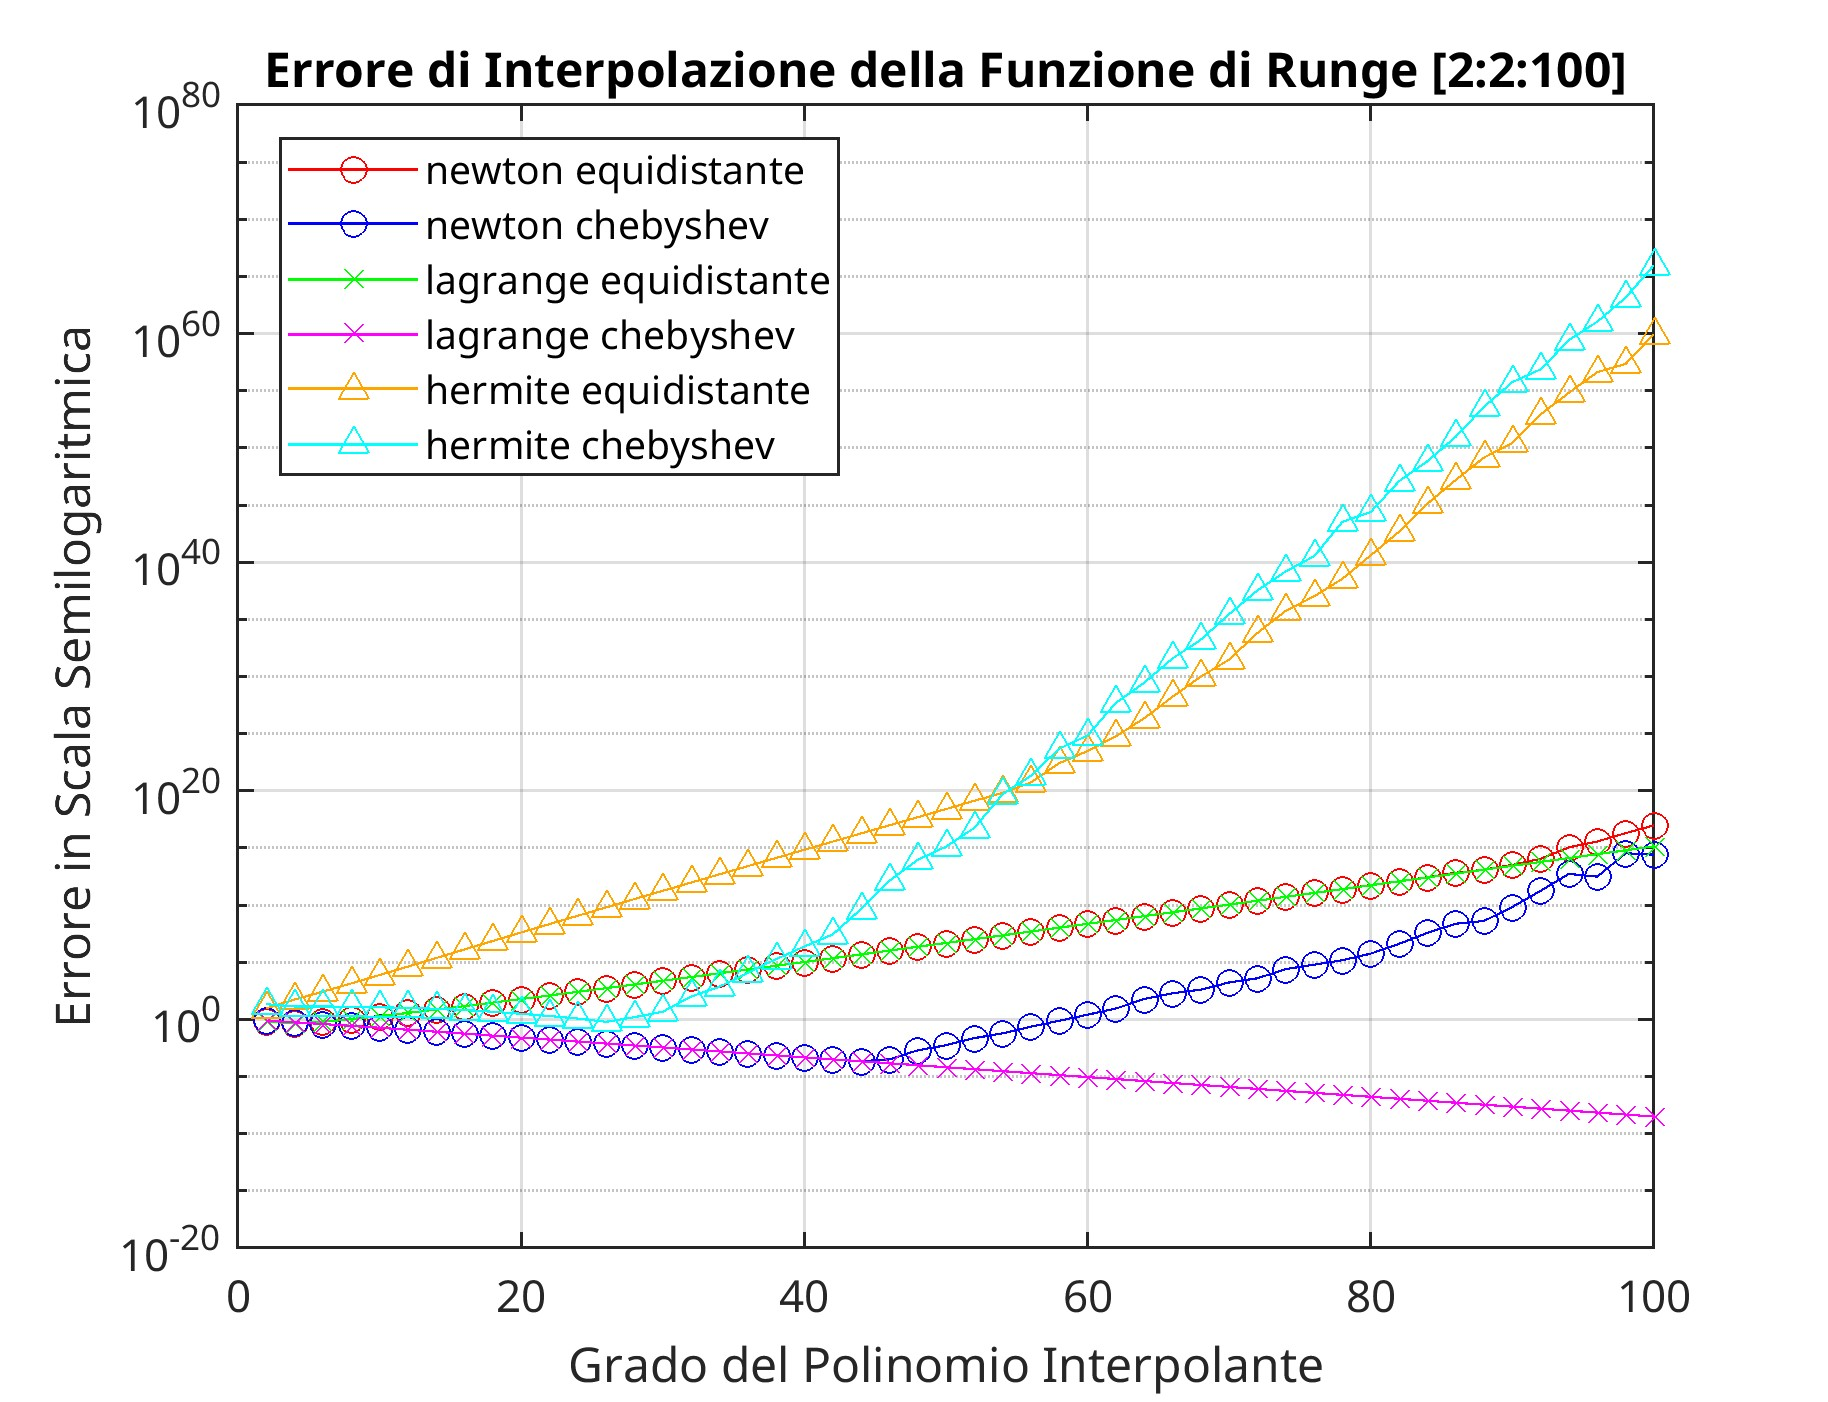
\includegraphics[width=0.9\textwidth]{../figure/plot21-1}  
\end{figure}
\begin{figure}[h!]
  \centering
  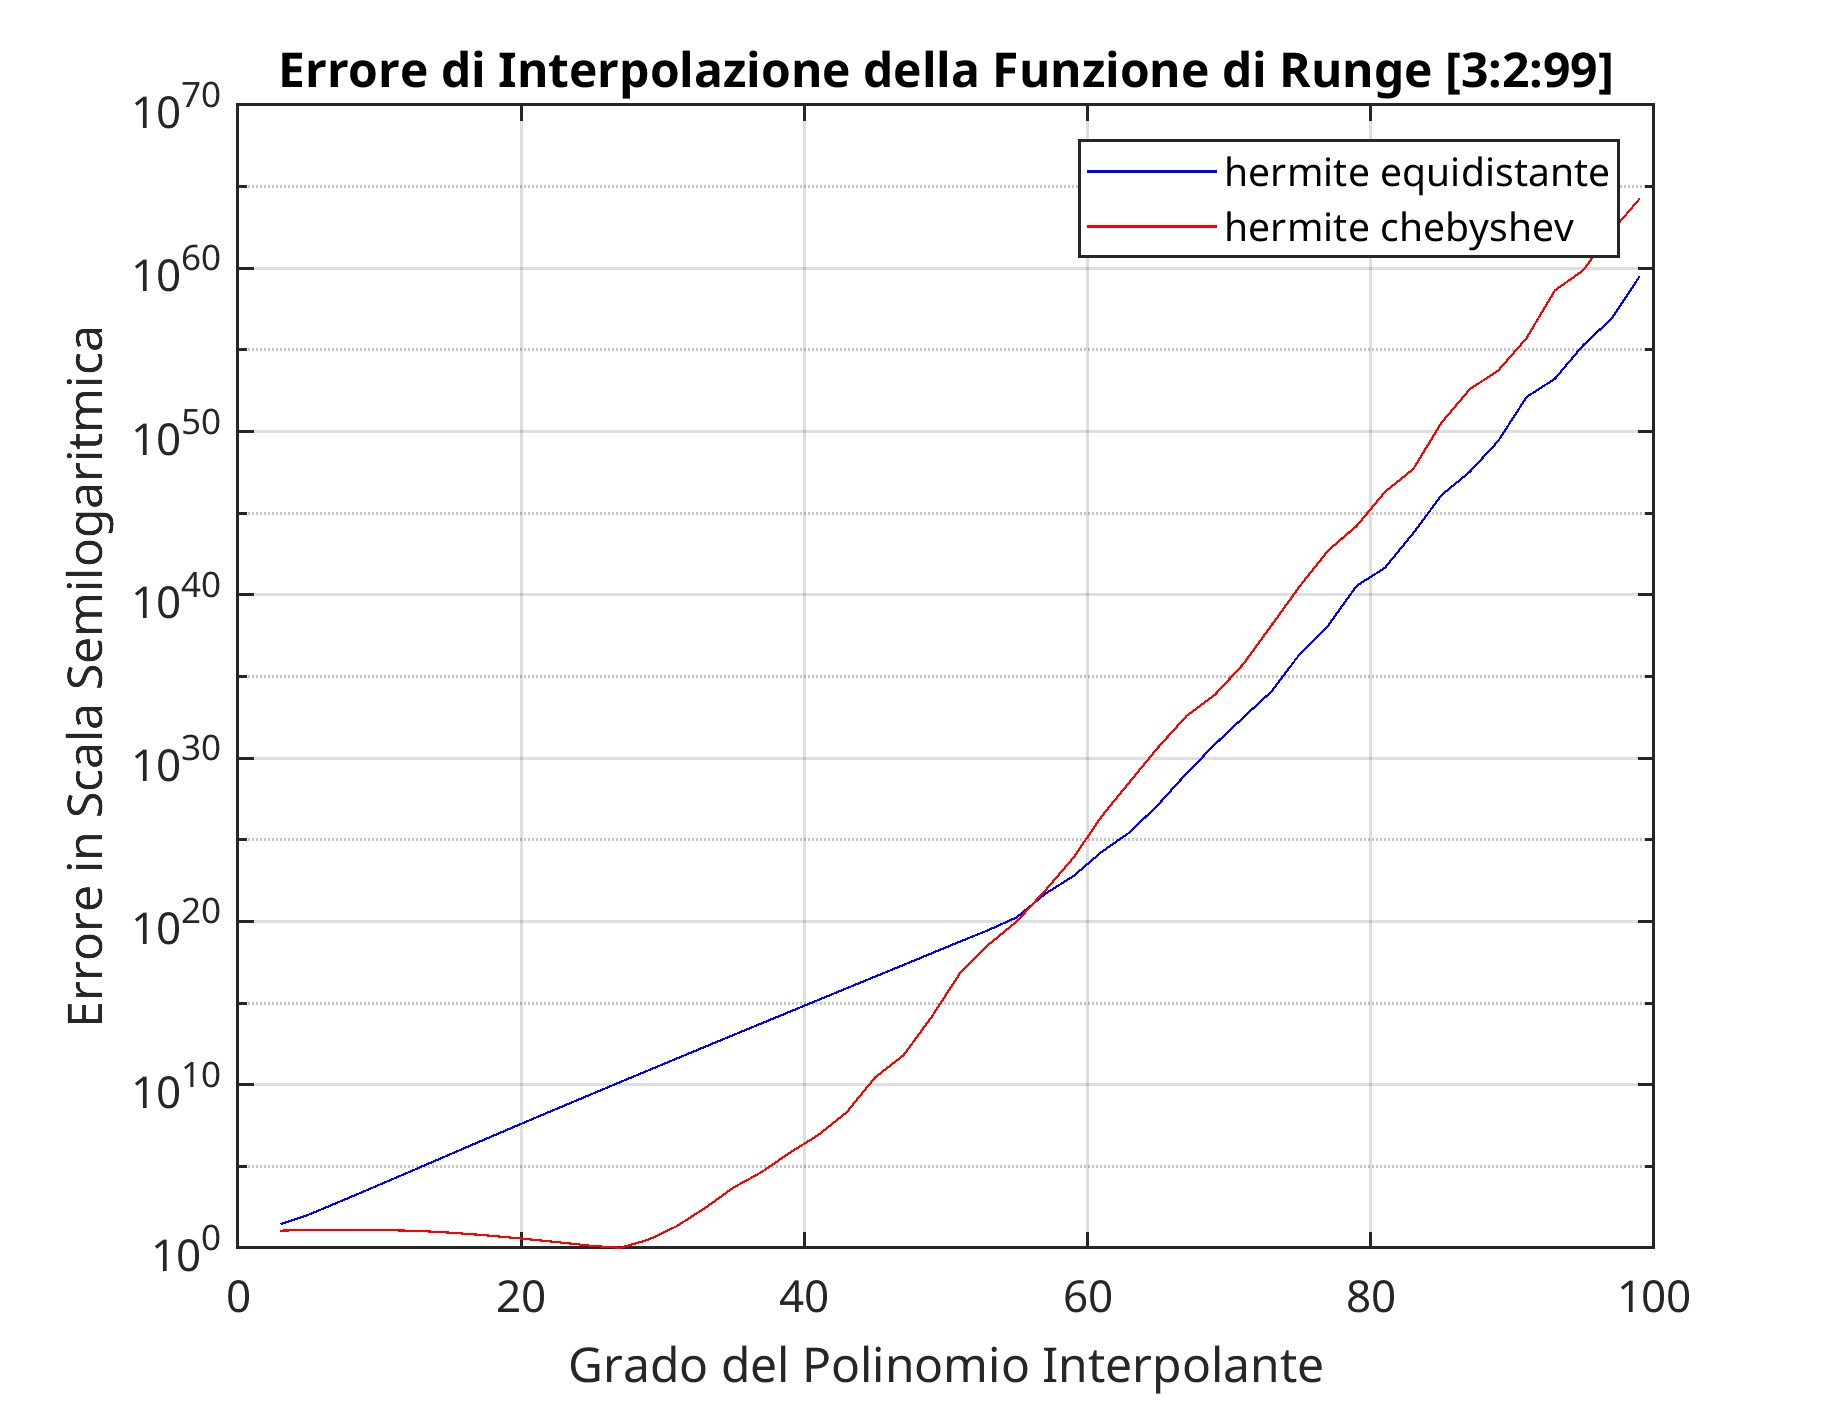
\includegraphics[width=0.9\textwidth]{../figure/plot21-2}  
\end{figure}
\newpage

\section{}
\lstinputlisting{../functions/22/myspline.m}
\section{}
\begin{figure}[h!]
  \centering
  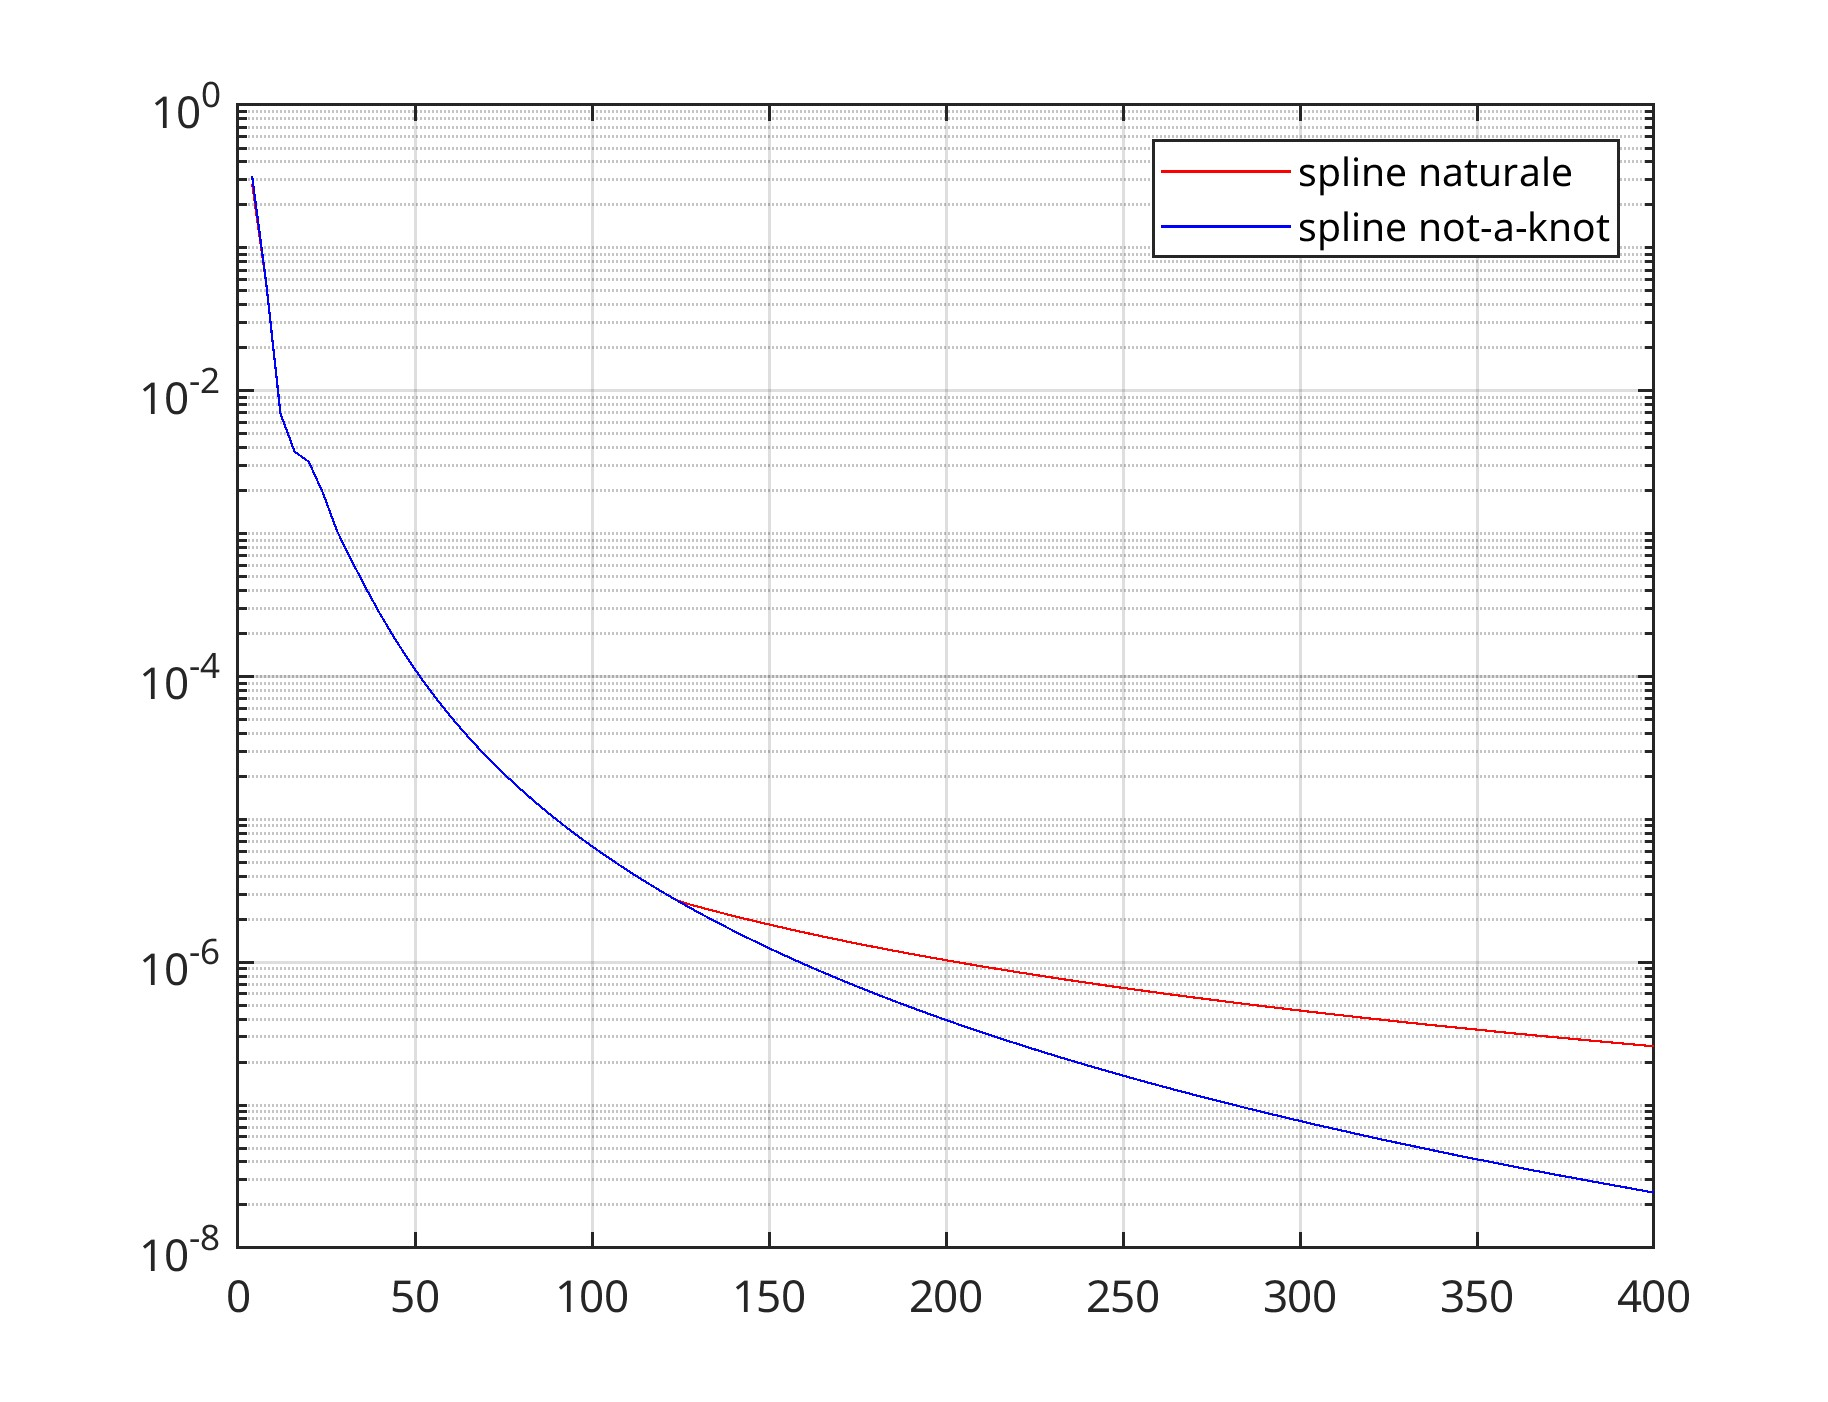
\includegraphics[width=0.9\textwidth]{../figure/esercizio_23}  
\end{figure}
\end{document}
